\documentclass[a4paper,utf8]{article}
\usepackage[heading,fancyhdr]{ctex}
\usepackage{amsmath,amssymb,geometry,lastpage,ulem}
\usepackage{array,tabularx,tabulary,mhchem,xspace}
\usepackage{floatrow,subfig,multirow,bigstrut}
\usepackage{siunitx,booktabs,longtable,graphicx,xfrac,nameref}
\lineskiplimit=1pt
\lineskip=3pt
\geometry{
    top=25.4mm, 
    left=25mm, 
    right=25mm, 
    bottom=25mm,
    headsep=5.9mm,
}
\ctexset{
    section = {format+=\raggedright}
}
\newcommand{\fgref}[1]{图~\ref{#1}\xspace}
\newcommand{\seqref}[1]{式~(\ref{#1})}
\newcommand{\expinfo}[7][无]{
    {\zihao{-3}\bfseries\songti
    实验名称:\uline{\hfill\mbox{#2}\hfill} \\[2.9mm]
    学\quad 号:\uline{\makebox[25mm]{#3}}\hfill
    姓\quad 名:\uline{\makebox[25mm]{#4}}\hfill
    班\quad 级:\uline{\makebox[25mm]{#5}} \\[2.9mm]
    合作者:\uline{\makebox[25mm]{#1}} \hfill
    桌\quad 号:\uline{\makebox[25mm]{#6}}\hfill\makebox[25mm+4em]{}\\[2.9mm]
    实验日期:\uline{\makebox[30mm]{#7}}\hfill\mbox{} \\[58.7mm]
    }
}
\newcommand{\pointingbox}{
    {\zihao{4}\bfseries\songti%
    实验考核\\[3mm]
    \extrarowheight=3mm
    \begin{tabularx}{150mm}{|X|X|X|X|X|}\hline
        \hfil 项目 \hfil  & \hfil 实验预习 \hfil & \hfil 实验过程 \hfil & \hfil 分析与讨论 \hfil & \hfil 总评 \hfil \\[3mm] \hline
        \hfil 评价 \hfil &  &  &  &  \\[3mm] \hline
    \end{tabularx}
    }
}
\newcommand{\derivative}[2]{\frac{\mathrm{d} #1}{\mathrm{d} #2}}
\newcommand{\thinking}[2]{\textbf{#1}\\
答:\begin{minipage}[t]{0.85\textwidth}
    #2
\end{minipage}}
\pagestyle{fancy}
\fancyhf{} \fancyhead[C]{电路基础实验} \fancyfoot[C]{\thepage~/~\pageref{LastPage}}
\newcounter{Rownumber}
\newcommand*{\Rown}{\stepcounter{Rownumber}\theRownumber}
\newcommand*{\resetRown}{\setcounter{Rownumber}{0}}
\newcommand{\qrange}[3]{\qtyrange[range-phrase = \text{$\sim$},range-units =single]{#1}{#2}{#3}}
\floatsetup[table]{capposition=top}
\newcolumntype{C}{>{\hfil}X<{\hfil}}
\renewcommand{\Nameref}[1]{\textbf{\ref{#1}~\nameref{#1}}} %导入导言
\usepackage{picinpar}
\newcommand*{\Usa}{$V_1$}
\newcommand*{\Usb}{$V_2$}
\begin{document}
\begin{center}
    {\mbox{}\\[7em]\zihao{2}\bfseries\songti%
    电路基础实验报告}\\[34mm]
    \expinfo[张泽钒]{基尔霍夫定律}{22301077}{张蕴东}{22高分子}{35}{2024.5.14}
\end{center}
\newpage
\section{实验目的}
\begin{enumerate}
    \item 加深对基尔霍夫定律的理解。
    \item 学习验证定律的方法和仪器仪表的正确使用。
\end{enumerate}

\section{实验原理}%简单描述,含必要的公式和附图;
    基尔霍夫定律是集总电路的基本定律,包括电流定律(KCL)和电压定律(KVL)。\par
    基尔霍夫定律规定了电路中各支路电流之间和各支路电压之间必须服从的约束关系,无论电路元件是线性的或是非线性的,时变的或是非时变的,只要电路是集总参数电路,都必须服从这个约束关系。

\section{实验仪表}
    RIGOL DM3058 万用表、RIGOL DP832 直流稳压电源、电路分析实验箱、导线若干。
\section{实验内容}
    \begin{enumerate}
        \item 验证(KCL)定律,即 $\sum i=0$。分别在自行设计的电路或参考的电路中,任选一个节点,测量流入流出该节点的各支路电流数值和方向。
        \item 验证(KVL)定律,即 $\sum u=0$。分别在自行设计的电路或参考的电路中任选一网孔(回路),测量网孔内所有支路的元件电压值和电压方向。
    \end{enumerate}
\section{实验结果与分析}
    在计算时并不会用到所有的测量值,故这里只选取了部分值用于计算,所有的测量结果在原始数据页展示。
    \subsection{线性对称电路 1}
        电路图如下: \par
        \begin{figure}[!ht]
            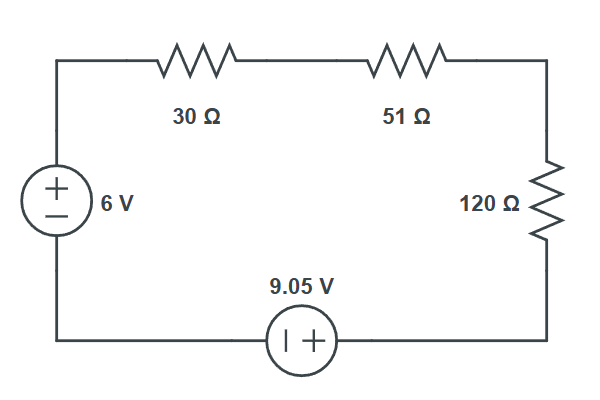
\includegraphics[width=0.5\textwidth]{cir1.png}
        \end{figure}\par
        此电路只有一条回路,只能验证 KVL 定律。根据测得数据验证:\par
        \begin{equation*}
            \sum U= 0.46+0.77+1.82+6-9=0.05\approx 0
        \end{equation*}\par
        考虑测量误差,可以认为 KVL 定律成立。

    \subsection{线性对称电路 2}
        电路图如下: \par
        \begin{figure}[!ht]
            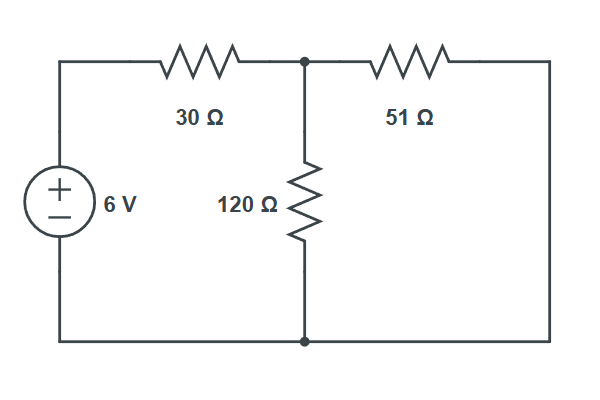
\includegraphics[width=0.5\textwidth]{cir2.png}
        \end{figure}\par
        在此电路中,选用左侧回路以及上方节点验证如下\par
        \begin{align*}
            \sum U&= 2.75+3.28-6=0.03\approx 0\\
            \sum I&= 91.7-64.3-27.3=0.1\approx 0
        \end{align*}\par
        考虑测量误差,可以认为基尔霍夫定律是正确的。

    \subsection{线性不对称电路}
        电路图如下: \par
        \begin{figure}[!ht]
            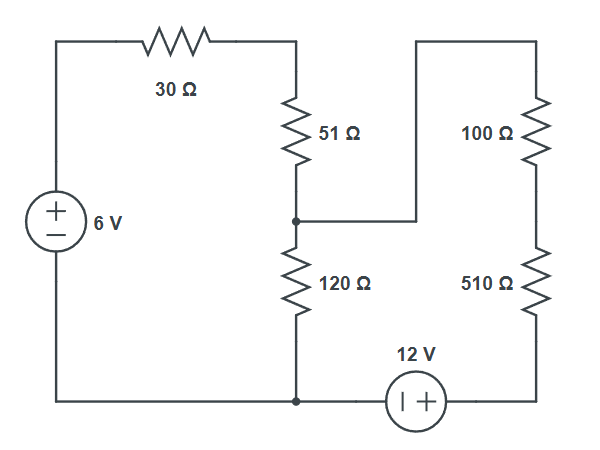
\includegraphics[width=0.5\textwidth]{cir3.png}
        \end{figure}\par
        在此电路中,选用左侧回路以及中间节点验证如下\par
        \begin{align*}
            \sum U&= 0.5+0.88+3.66-5=-0.04\approx 0\\
            \sum I&= 30.6-16.8-13.7=0.1\approx 0
        \end{align*}\par
        考虑测量误差,可以认为基尔霍夫定律是正确的。

    \subsection{非线性对称电路}
        电路图如下: \par
        \begin{figure}[!ht]
            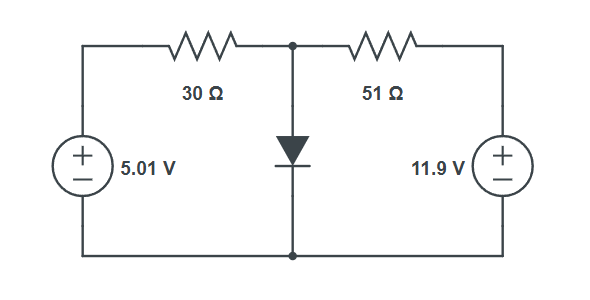
\includegraphics[width=0.5\textwidth]{cir4.png}
        \end{figure}\par
        在此电路中,选用左侧回路以及上方节点验证如下\par
        \begin{align*}
            \sum U&= 3.80+1.21-5.01=0\\
            \sum I&= 141.8-47.1-94.4=0.3\approx 0
        \end{align*}\par
        考虑测量误差,可以认为基尔霍夫定律是正确的。

    \subsection{非线性不对称电路}
        电路图如下: \par
        \begin{figure}[!ht]
            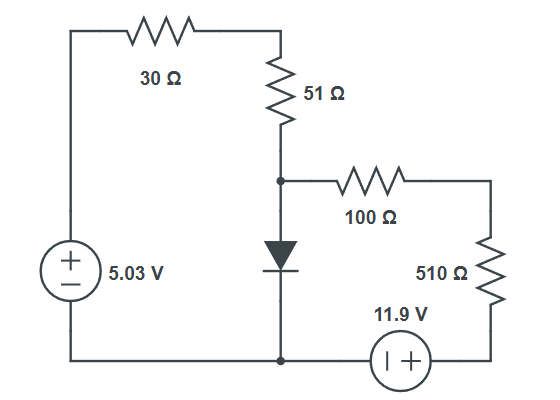
\includegraphics[width=0.5\textwidth]{cir5.png}
        \end{figure}\par
        在此电路中,选用左侧回路以及中间节点验证如下\par
        \begin{align*}
            \sum U&= 1.52+0.90+2.61-5.03=0\\
            \sum I&= 50.8+18.0-68.8=0
        \end{align*}\par
        考虑测量误差,可以认为基尔霍夫定律是正确的。

    \subsection{结果分析}
        在本次实验的五个不同的电路中,无论是对称电路还是非对称电路,又或者是非线性电路,测得的节点电流和回路电压代数和都接近零。这跟基尔霍夫定律所描述的情况完全一致,可以认为基尔霍夫定律成立。

\section{思考题}
    \subsection{什么是基尔霍夫定律,包括两个什么定律?}
        基尔霍夫定律包括两个定律:
        \begin{enumerate}
            \item 基尔霍夫电流定律(KCL):该定律表明,在任何一个电路节点(或接点),流入节点的电流之和等于流出节点的电流之和。这一规律反映了电荷守恒原理。
            \item 基尔霍夫电压定律(KVL):该定律表明,在一个闭合电路回路中,各个元件的电压之和等于零。这一规律反映了能量守恒原理。
        \end{enumerate}
    \subsection{基尔霍夫定律适用于什么性质元件的电路?}
        基尔霍夫定律建立在电荷守恒定律、欧姆定律及电压环路定理的基础之上,在稳恒电流条件下严格成立。因此运用基尔霍夫定律进行电路分析,仅与电路的连接方式有关,而与构成该电路的元器件具有什么样的性质无关。它除了可以用于直流电路的分析,和用于似稳电路的分析,还可以用于交流电路的分析。不过此时要考虑磁场的影响,情况略微复杂。这是因为能量不再完全以电场能的方式存在,同时也会有磁场能。
    \subsection{测试中,如果使用的电流表内阻较大,为 \SI{30}{\ohm},电压表内阻较小,为 \SI{200}{\ohm}时,试分析对测量结果有何影响?}
        本次实验采用了电流表外接法,因此如果电流表的内阻较大,当它接入电路时,会增加电路的总电阻,从而减小通过电路的电流。这会导致测量电流偏小。如果电压表的内阻较小,当它接入电路时,会分流部分电流,从而降低被测点的电压。这会导致测量电压也偏小。
\section{实验心得}
    此次实验使用了 5 个电路来验证基尔霍夫电路定律,在实际操作中,观察到了由于仪器误差和连接线电阻带来的微小偏差,但总体上实验结果符合理论预期。同时在实验之后我也自己用软件模拟了这些电路,对未分析节点和回路重新验证了一次,再一次证明定律成立。这些实验不仅加深了对基尔霍夫定律的理解,也提升了在实际电路中应用这些定律的能力。
    
\section{原始数据}
    \begin{center}\begin{figure*}
        \subfloat[1]{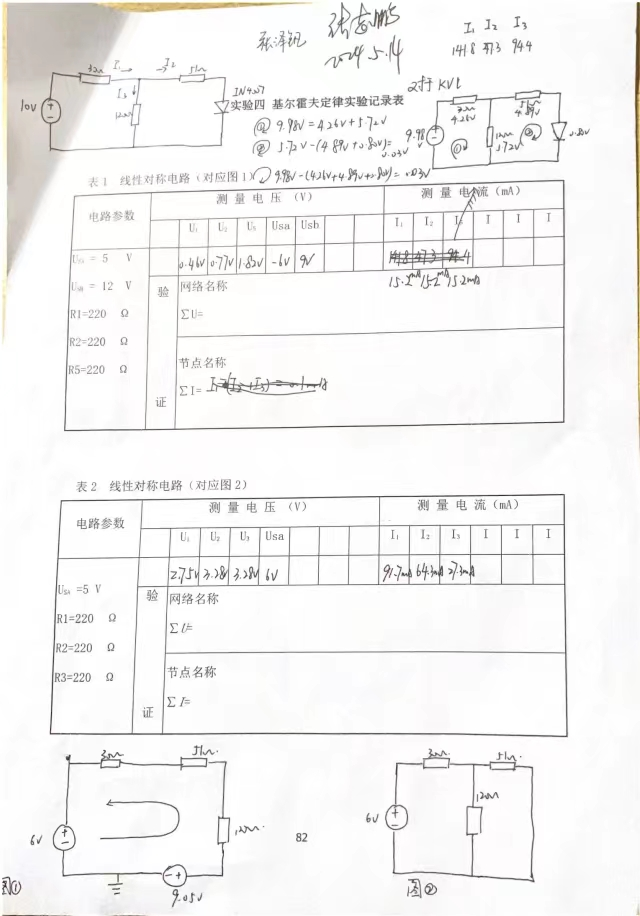
\includegraphics[width=0.45\textwidth]{data1.jpg}}
        \subfloat[2]{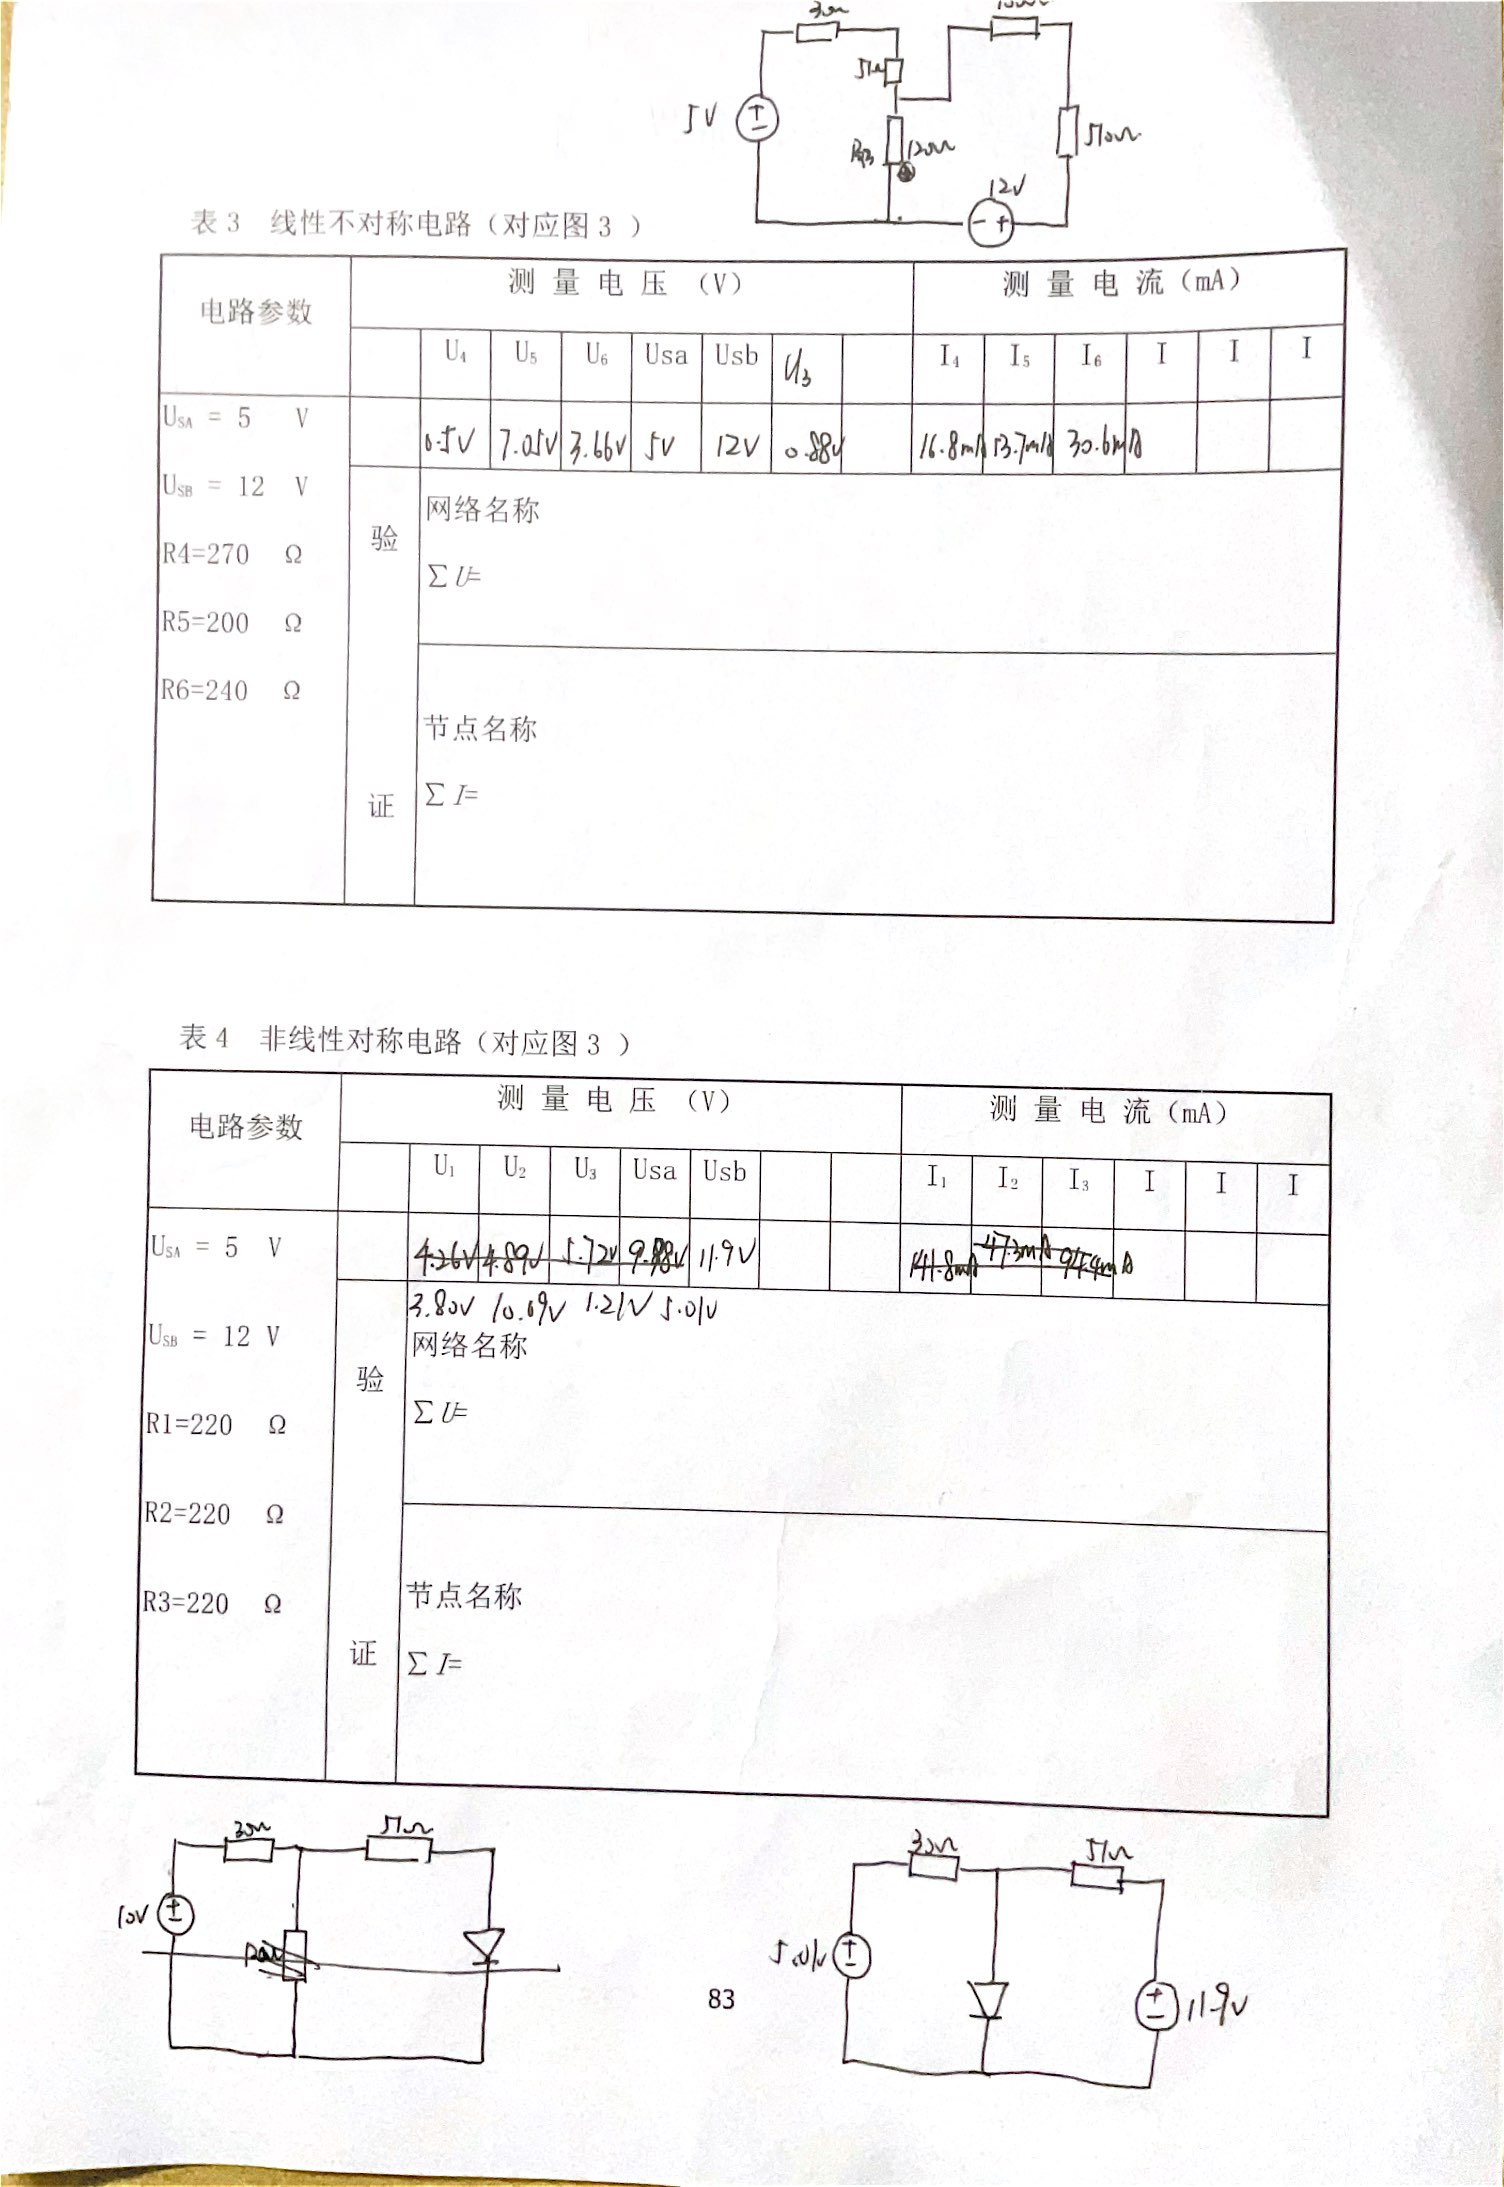
\includegraphics[width=0.45\textwidth]{data2.jpeg}}\\
        \subfloat[3]{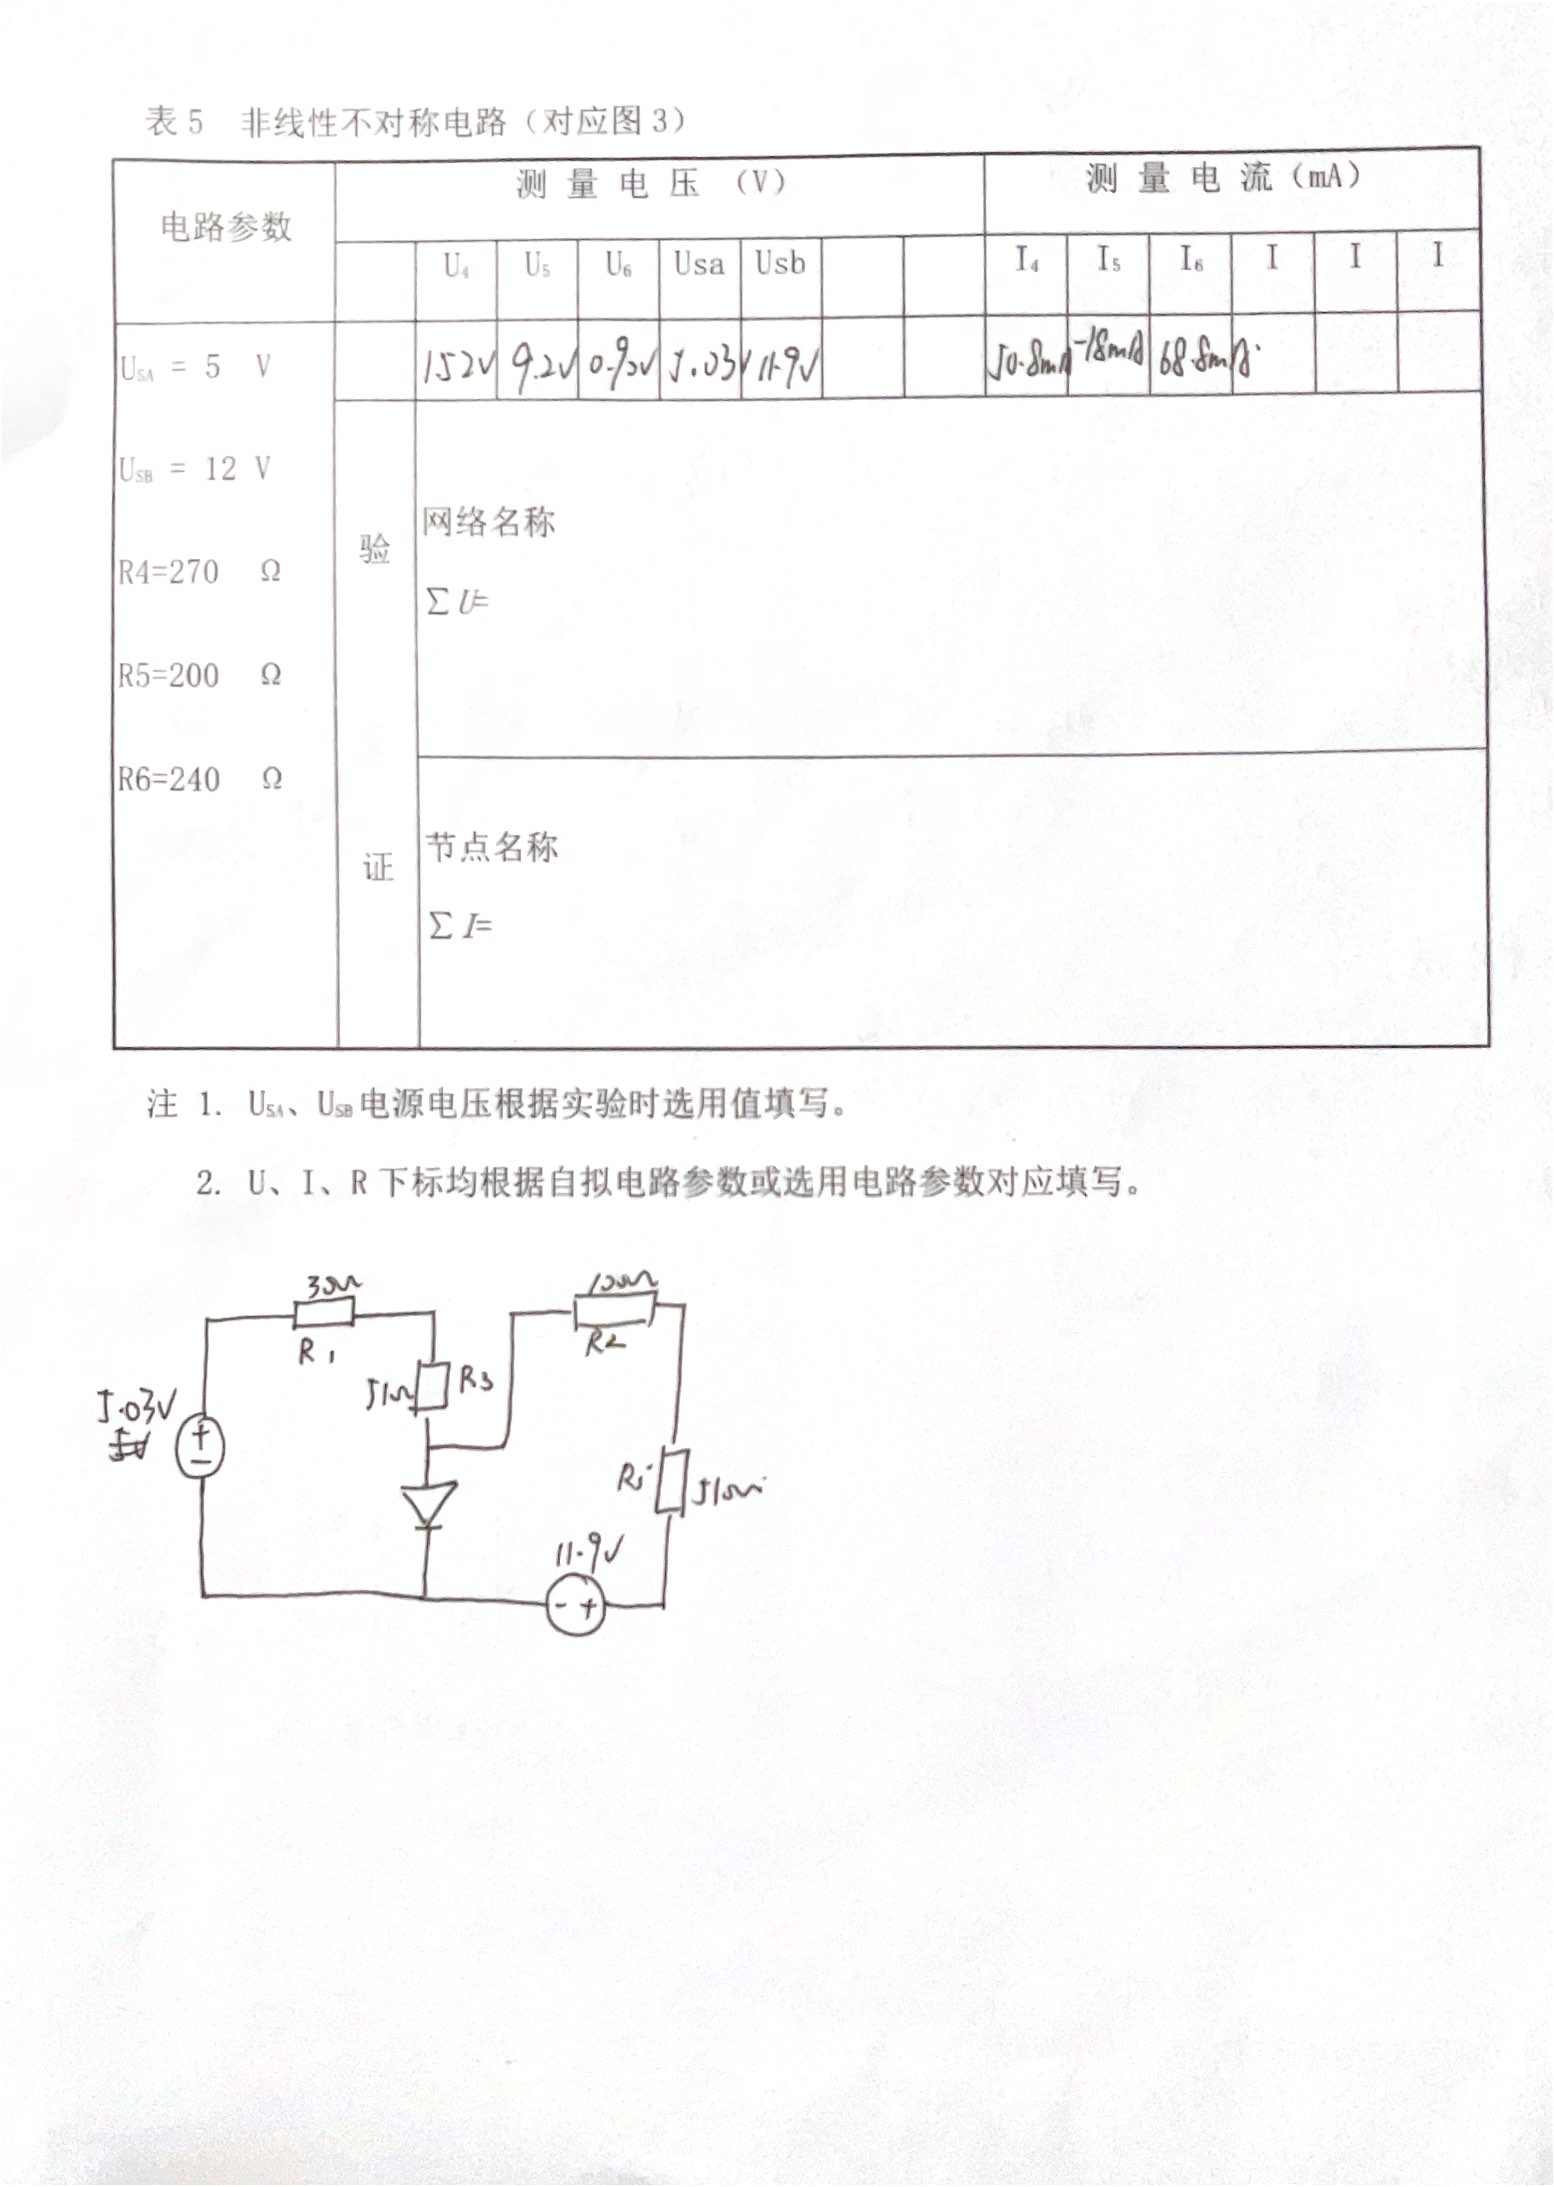
\includegraphics[width=0.45\textwidth]{data3.jpeg}}
    \end{figure*}
    \end{center}

\end{document}